\documentclass{article}
\usepackage[ngerman]{babel}
\usepackage[utf8]{inputenc}
\usepackage{graphicx} 
\usepackage{svg}
\graphicspath{{Bilder/}}
\usepackage{geometry}
\usepackage{amsmath}
\usepackage{pdflscape}
\geometry{a4paper, top=25mm, left=30mm, right=25mm, bottom=20mm}
\begin{document}

\renewcommand{\rmdefault}{phv}
\renewcommand{\sfdefault}{phv}
\renewcommand{\arraystretch}{1.1}

\section{Inbetriebnahme der Sensor}
Die Werte $\phi_K$, $\dot{\phi_K}$ und $\ddot{\phi_K}$ müssen für die Regelung des Würfels erfasst werden. Hierfür wird das Bauteil \textit{2020 Adafruit Industries} verwendet. Dieser Chip verfügt über einen Beschleunigungssensor, ein Gyroskop und Magnetometer, welche jeweils über drei Achsen die Beschleunigung, die Winkelgeschwindigkeit und die magnetische Flussdichte messen. 
Um die Sensoren in das Gesamtsystem einzubinden müssen diese über $I^2C$ mit der Rechnereinheit verbunden und kalibriert werden. Außerdem müssen die gemessenen Werte in die benötigten Größen überführt werden.

\subsection{Verwendete Koordinatensysteme}
Bei der Betrachtung der Würfels werden zwei Koordinatensysteme verwendet. Das Weltkoordinatensystem $(x_w, y_w, z_w)^T$ beginnt im Drehpunkt der Würfelseite und ist fix. Das Würfelkoordinatensystem $(x, w, y)^T$ beginnt ebenfalls im Drehpunkt allerdings rotiert es mit dem Winkel $\phi_K$, welcher die relative Rotation der Würfelsystem zum Weltkoordinatensystem beschreibt. An der Außenseite des Würfels sind die beiden Sensoren befestigt, an der Innenseite sind die Schwungmasse, der Motor und die Bremse angebracht. Die Achsen der Sensorkoordinatensysteme liegen parallel zu den Würfelkoordinaten. Die Translation entspricht der Position des Sensors zum Drehpunkt und somit zum Ursprung des Würfelkoordinatensystem.

\begin{figure}[h]
	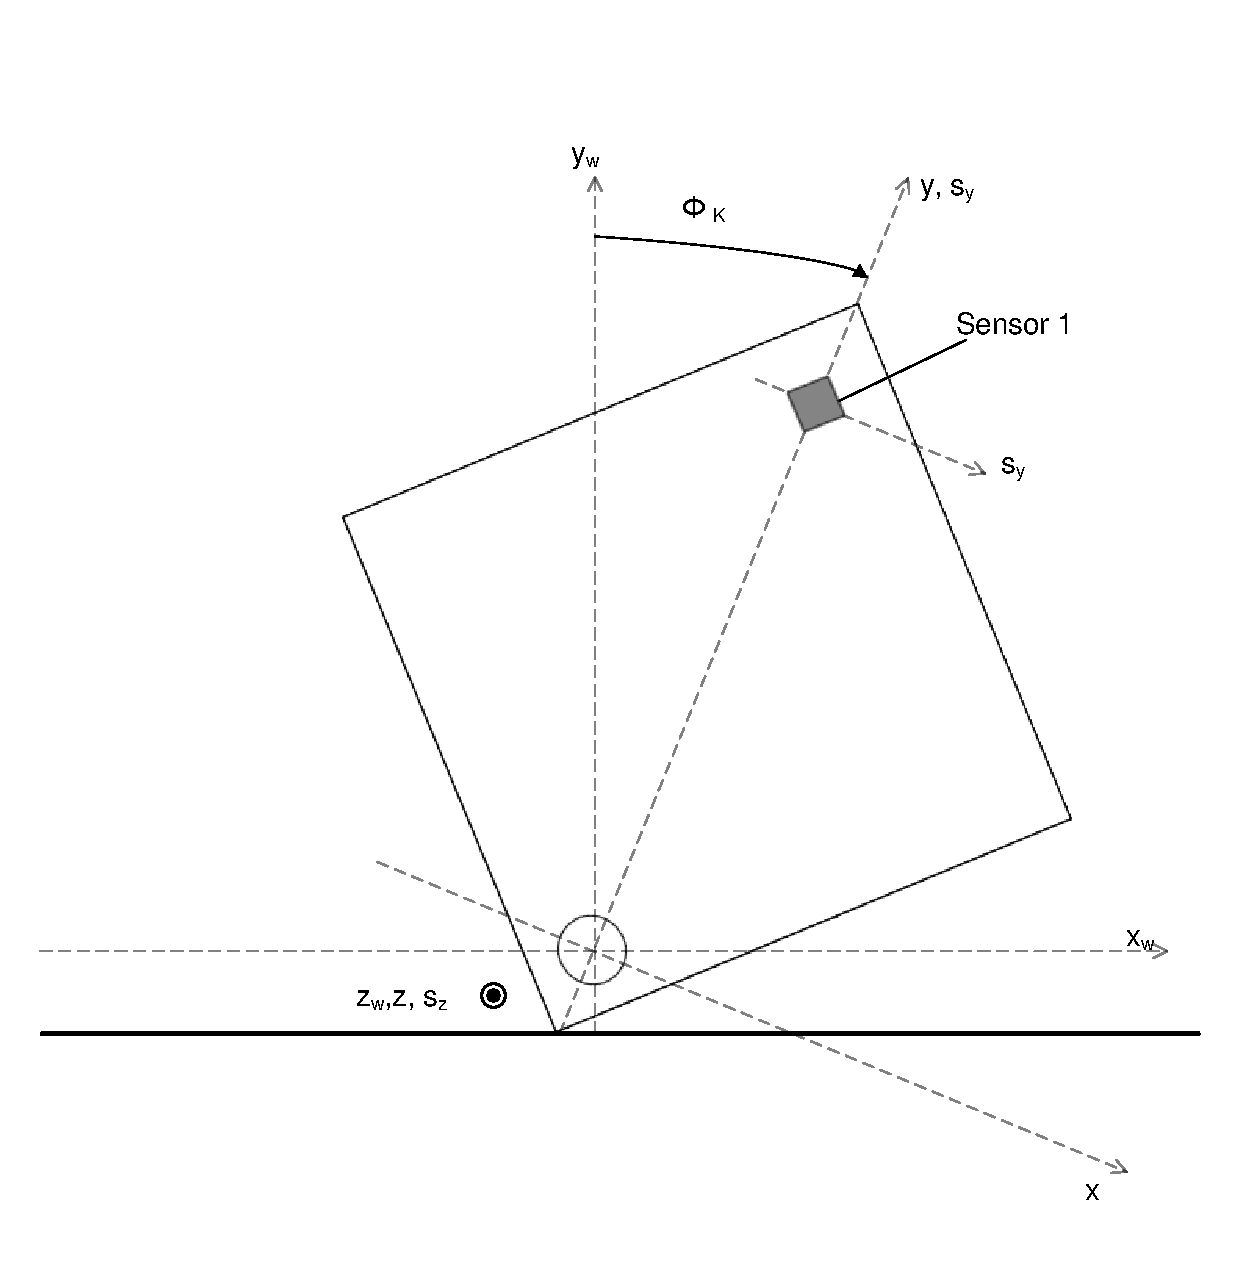
\includegraphics[width=\linewidth]{Koordinatensystem}
	\caption{Darstellung Koordinatensysteme, Quelle: eigene Darstellung}
\end{figure}

Sensorkoordinaten in Winkelkoordinaten umwandeln, welche Sensorachsen müssen invertiert werden?
Letze Messsung/Kalibrierung : x- und y-Achse invertiert, z-Achse nicht invertiert, allerdings ist die Richtung der z-Achse irrelevant da cosinus symmetrisch ist

\subsection{Anbindung über $I^2C$ und Sensorkonfiguration}
Der Sensor unterstützt das $I^2C$ Protokoll bei einer Frequenz von $400k Hz$. Mit Hilfe der Registeradressen des Sensors, welche im Datenblatt dokumentiert sind, werden die aktuellen Sensorwerte ausgelesen und Konfigurationen festgelegt werden.

Der Beschleunigungssensor erfasst Beschleunigungen im Bereich von $\pm2 g$ mit einer Auflösung von $0.061 mg / LSb$. Die Winkelgeschwindigkeit des Gyroskop bewegt sich in einem Bereich von $\pm 245 dps$ mit einer Auflösung von $8.75 mdps / LSb$. Der Magnetometer liefert Werte im Bereich von $\pm 2gauss$ und bringt hierbei eine Auflösung von $0.08 mgauss / LSb$.

\subsection{Ermittlung der Größen $\phi_K$, $\dot{\phi_K}$ und $\ddot{\phi_K}$}
Die Sensoren erfassen die jeweilige Größe in drei Achsen. Betrachtet man die Drehbewegung der Würfelseite, so entspricht die Y-Achse des Sensors der Radialachse des Würfels und die X-Achse des Sensors der Tangentialachse der Drehbewegung. Die Z-Achse des Sensors steht senkrecht auf der Drehebene.

\subsubsection{Bestimmung von $\phi_K$}
Der Beschleunigungssensor erfasst die drei Beschleunigungswerte in $g$ bzw. in der SI-Einheit $\frac{m}{s^2}$. Aus den X- und Y-Werten kann die aktuelle Winkelbeschleunigung $\ddot{\phi_K}$ bestimmt werden. Hierbei muss beachtet werden, dass der Sensor in Ruhelage eine absolute Beschleunigung von $1g$ ausgibt, also offset-behaftet ist. Die Zusammensetzung der Beschleunigungswerte kann winkelabhängig bestimmt werden.

\[\ \ddot{x_S} := Beschleunigungswert \ in \ X \ in \ \frac{m}{s^2} \]
\[\ \ddot{y_S} := Beschleunigungswert \ in \ Y \ in \ \frac{m}{s^2} \]
\[\ \ddot{z_S} := Beschleunigungswert \ in \ Z \ in \ \frac{m}{s^2} \]
\[\ r_S := Abstand \ von  \ Sensor \ zu \ Drehpunkt \]

\[\ (\ddot{x_S}, \ddot{y_S}, \ddot{z_S}) = (r_S \cdot \ddot{\phi_K} + sin(\phi_K) \cdot g , -r_S \cdot {\dot{\phi_K}}^2 - cos(\phi_K) \cdot g , 0) \]

\[\ \ddot{\phi_K} = \frac{\ddot{x_S} - sin(\phi_K) \cdot g }{r_S} \]

\subsubsection{Bestimmung von $\dot{\phi_K}$}
Das Gyroskop gibt die Winkelgeschwindigkeiten in Grad pro Sekunde wider. Somit muss der Z-Wert lediglich in SI-Einheiten umgewandelt werden.

\[\ {\omega_S} := Winkelgeschwindigkeit \ um \ Z \ in \ Grad \ pro \ Sekunde \]

\[\ \dot{\phi_K} = {\omega_S} \cdot \frac{2 \cdot \pi}{360} \]

\subsubsection{Bestimmung von $\phi_K$}
Der Ausfallwinkel des Würfels kann über verschiedene Wege ermittelt werden. Nach der Kalibrierung des Magnetometer kann über das Verhältnis der magnetischen Flussdichte in X- und Y-Richtung der Winkel berechnet werden. Dieses Verfahren hat sich allerdings als extrem störanfällig bewiesen und ist somit für diesen Anwendungsfall untauglich.

Über die folgende Differenzialgleichung zur Bestimmung des dynamischen Verhalten des Systems kann der Winkel $\phi_K$ berechnet werden.

\[\ (\Theta_K^{(A)} + m_w \cdot l^2) \cdot \ddot{\phi_K} = (m_K  l_K + m_w \cdot l) \cdot g \cdot sin(\phi_K)) - C_K \cdot \dot{\phi_w} - T_M  \]

\[\ sin(\ddot{phi_K}) = (\Theta_K^{(A)} + m_w \cdot l^2) \cdot \ddot{\phi_K} + C_K \cdot \dot{\phi_w} + T_M \]

Die Sensoren liefern die Werte $\ddot{\phi_K}$ und $\dot{\phi_K}$, die Winkelgeschwindigkeit $\dot{\phi_R}$ wird über den Motortreiber ermittelt. Somit kann $\phi_K$ mittels der obigen Gleichung berechnet werden. Allerdings müssen die konstanten Werte bereits bestimmt worden sein. Folglich kann diese Methode erst nach erfolgreicher Systemidentifikation verwendet werden.

Um die Systemidentifikation durchzuführen wird ein zweiter Sensor an der Würfelseite angebracht. Über das Verhältnis der Abstände der Sensoren zum Drehpunkt und deren Beschleunigungswerte kann eine Winkelschätzung durchgeführt werden. Mit diesem Prinzip können die Systemparameter bestimmt werden und anschließend die oben genannte Methode verwendet werden. Dadurch ist der zweite Sensor lediglich zur Systemidentifikation notwendig.

\[\ r_S1 := Abstand \ von \ Sensor \ 1 \ zu \ Drehpunkt \]
\[\ r_S2 := Abstand \ von \ Sensor \ 2 \ zu \ Drehpunkt \]
\[\ \mu = \frac{r_{S1}}{r_{S2}} \]

\[ \ddot{x}_{S1} - \mu \cdot \ddot{x}_{S2} = (1 - \mu) \cdot g \cdot sin(\phi_K) \]

\[\ \ddot{y}_{S1} - \mu \cdot \ddot{y}_{S2} = - (1 - \mu) \cdot g \cdot cos(\phi_K) \]

\[\ \frac{\ddot{x}_{S1} - \mu \cdot \ddot{x}_{S2}}{\ddot{y}_{S1} - \mu \cdot \ddot{y}_{S2}} = 
-tan(\phi_K) \]

\[\ \phi_K = - atan(\frac{\ddot{x}_{S1} - \mu \cdot \ddot{x}_{S2}}{\ddot{y}_{S1} - \mu \cdot \ddot{y}_{S2}}) \]


\subsection{Kalibrierung der Sensoren}
Die erforderlichen Sensorwerte um die benötigten Größen zu bestimmen sind $\ddot{x}_S$, $\ddot{y}_S$ und $\omega_S$. Die Sensoren geben die physikalischen Größen in 16-Bit-Werten in der Zweierkomplement-Darstellung wieder. Über einen Faktor kann der entsprechende Wert als SI-Einheit dargestellt werden. Bei der Kalibrierung muss der Offset zwischen Sollausgabe und Istwert ermittelt werden, um die Sensorwerte korrigieren zu können.

\subsubsection{Kalibrierung des Beschleunigungssensor}
In der Ruhelage soll der Sensor einen Beschleunigungsbetrag von $1g$ anzeigen. Im ersten Aufbau wird der Sensor so positioniert, dass die Gravitation lediglich den X-Wert beeinflusst, folglich ist der Sollwert der X-Beschleunigung $1g$. Um die mittlere Abweichung $\ddot{x}_{off}$ zu ermitteln wird eine Messreihe von $m = 10000$ Messwerten aufgezeichnet. 

\[\ \ddot{x}_{off} = 1g - \frac{\sum_{i = 1}^{m}}{m} \ddot{x} \]

Die oben berechnete Abweichung bezieht sich auf die Darstellung des Wertes als SI-Einheit. Um den Offset in Ganzzahldarstellung zu ermitteln muss durch den Umrechnungsfaktor dividiert und gerundet werden.

\[\ \ddot{x}_{off}^{int} = \frac{\ddot{x}_{off}}{factor} \]

Die Bestimmung der Abweichung der Beschleunigung für die Y-Achse verläuft analog.

\subsubsection{Kalibrierung des Gyroskop}
Der Sollwert des Gyroskop in der Ruhelage beträgt $0 dps$. Somit lässt sich der Offset analog zu dem Beschleunigungssensor ermitteln.

\subsubsection{Messergebnis für X-Achse des Beschleunigungssensor}
Die Messung zur Bestimmung des Offset der X-Achse wurde zweimal durchgeführt. Zuerst wurde die X-Achse des Sensor in Gravitationsrichtung gestellt. Bei dem zweiten Durchlauf zeigte sie entgegen der Gravitationsrichtung.

\[\ Messung \ X-Achse \ Beschleunigungssensor \ in \ Gravitationsrichtung \]
\[\ Durchgefuehrt \ am \ 10.05.2016 \]
\[\ Anzahl \ Messungen : m = 10000 \]
\[\ \frac{\sum_{i = 1}^{m} \ddot{x}^{int}}{m} = -19770 \]
\[\ \frac{\sum_{i = 1}^{m} \ddot{x}}{m} = -1.0966 \]
\[\ \ddot{x}_{off}^{int} = 34371 \]
\[\ \ddot{x}_{off} = 2.0966 \]

\[\ Messung \ X-Achse \ Beschleunigungssensor \ gegen \ Gravitationsrichtung \]
\[\ Durchgefuehrt \ am \ 10.05.2016 \]
\[\ Anzahl \ Messungen : m = 10000 \]
\[\ \frac{\sum_{i = 1}^{m} \ddot{x}^{int}}{m} = 15057 \]
\[\ \frac{\sum_{i = 1}^{m} \ddot{x}}{m} = 0.9185 \]
\[\ \ddot{x}_{off}^{int} = 1336 \]
\[\ \ddot{x}_{off} = 0.0815 \]

Die Ergebnisse zeigen, dass die Achsen auf dem Chip falsch markiert sein. Die Richtung kann allerdings problemlos korrigiert werden.

\subsubsection{Messergebnis für Y-Achse des Beschleunigungssensor}
Die Messung wurde analog zu der X-Achse zweimal durchgeführt. Die aufgezeichnete Sensorachse ist ebenfalls invertiert.

\[\ Messung \ Y-Achse \ Beschleunigungssensor \ in \ Gravitationsrichtung \]
\[\ Durchgefuehrt \ am \ 10.05.2016 \]
\[\ Anzahl \ Messungen : m = 10000 \]
\[\ \frac{\sum_{i = 1}^{m} \ddot{y}^{int}}{m} = -16085 \]
\[\ \frac{\sum_{i = 1}^{m} \ddot{y}}{m} = -0.9812 \]
\[\ \ddot{y}_{off}^{int} = 32479 \]
\[\ \ddot{y}_{off} = 1.9812 \]


\[\ Messung \ Y-Achse \ Beschleunigungssensor \ gegen \ Gravitationsrichtung \]
\[\ Durchgefuehrt \ am \ 10.05.2016 \]
\[\ Anzahl \ Messungen : m = 10000 \]
\[\ \frac{\sum_{i = 1}^{m} \ddot{y}^{int}}{m} = 16293 \]
\[\ \frac{\sum_{i = 1}^{m} \ddot{y}}{m} = 0.9939 \]
\[\ \ddot{y}_{off}^{int} = 100 \]
\[\ \ddot{y}_{off} = 0.0061 \]

\subsubsection{Messergebnis für die Z-Achse des Gyroskop}
Die Messung zur Bestimmung des Offset der Z-Achse wurde einmal durchgeführt.

\[\ Messung \ Z-Achse \ Gyroskop\]
\[\ Durchgefuehrt \ am \ 10.05.2016 \]
\[\ Anzahl \ Messungen : m = 10000 \]
\[\ \frac{\sum_{i = 1}^{m} {\omega}^{int}}{m} = 55 \]
\[\ \frac{\sum_{i = 1}^{m} {\omega}^{dps}}{m} = 0.4793 \]
\[\ {\omega}_{off}^{int} = -55 \]
\[\ {\omega}_{off} = -0.4793 \]

\subsection{Übertragung auf das 1D-Würfelmodell}
Die Übertragung der Kalibrierungswerte auf den eindimensionalen Prototyp ergab in den Testmessungen große Fehler. Der Test ergab einerseits, dass die Sensoren einzeln kalibriert werden müssen, da eine starke Abweichung zwischen den einzelnen Exemplaren herrscht. Andererseits führt der 3D-Druck des Prototyps zu einem Kippwinkel in Richtung der Z-Achse. Folglich muss das Modell zur Werteberechnung um einen Freiheitsgrad erweitert werden.

\subsection{Bestimmen der Werte in einem Modell mit zwei rotatorsichen Freiheitsgraden}
Die oben aufgezeigte Bestimmung der Werte $phi_K$, $\dot{\phi_K}$, $\ddot{\phi_K}$ wurde unter der Annahme durchgeführt, dass der von dem Winkel $\phi_K$ beschriebene rotatorische Freiheitsgrad beachtet werden muss. Allerdings ergibt sich durch die Qualität des 3D-Drucks ein nicht zu vernachlässigender Kippwinkel in Richtung der Z-Achse. Somit muss ein weiterer rotatorischer Freiheitsgrad beachtet werden, welcher von dem Winkel $\Theta_K$ beschrieben wird.

Unter der Annahme das keine Kraft außer der Gravitation wirkt, wird die Beschleunigung in Würfelkoordinaten wie folgt beschrieben werden.

\begin{equation}
\begin{array}{lclcl}
s_i 
& = & 
\begin{pmatrix} \ddot{x}^s_{i} \\ \ddot{y}^s_i \\ \ddot{z}^s_i \end{pmatrix}
& = &
\begin{pmatrix} 
g \cdot sin(\phi_K) \cdot cos(\Theta_K) \\
-g \cdot cos(\phi_K) \cdot cos(\Theta_K) \\
g \cdot sin(\Theta_K)
\end{pmatrix}
\end{array}
\end{equation}

Der Betrag des Beschleunigungsvektor muss stets gleich $1g$ sein, an Hand dieser Bedingung kann das obige LGS überprüft werden.

\begin{equation}
\begin{array}{lcl}
a^2 
& = &
\ddot{x}^2_i + \ddot{y}^2_i + \ddot{z}^2_i \\
 & = &
g^2 \cdot ( sin^2(\phi_K) \cdot cos^2(\Theta_K) + cos^2(\phi_K) \cdot cos^2(\Theta_K) + sin^2(\Theta_K) ) \\
& = &
g^2 \cdot ( cos^2(\Theta_K) \cdot (sin^2(\phi_K) + cos^2(\phi_K) ) + sin^2(\Theta_K) ) \\
& = &
g^2 \cdot (cos^2(\Theta_K) + sin^2(\Theta_K)) = g^2
\end{array}
\end{equation}

Die obigen Gleichungssysteme beschreiben die Dynamik des Prototyp ohne weitere Einflüsse wie z.B. das durch den Motor verursachte Drehmoment.

\begin{equation}
\begin{array}{lclcl}
s_i 
& = & 
\begin{pmatrix} \ddot{x}^s_i \\ \ddot{y}^s_i \\ \ddot{z}^s_i \end{pmatrix}
& = &
\begin{pmatrix} 
g \cdot sin(\phi_K) \cdot cos(\Theta_K) + \ddot{\phi}_K \cdot r_i \\
-g \cdot cos(\phi_K) \cdot cos(\Theta_K) - \dot{\phi}^2_K \cdot r_i - \dot{\Theta}^2_K \cdot r_i \\
g \cdot sin(\Theta_K) + \ddot{\Theta}_K \cdot r_i
\end{pmatrix}
\end{array}
\end{equation}

\subsubsection{Winkelschätzung mit zwei Freiheitsgraden}
Durch den zweiten Freiheitsgrad wird die Winkelschätzung von $\Theta_K$ und dessen Ableitungen beeinflusst. 

\begin{equation}
\begin{array}{lclcl}
s_i 
& = & 
\begin{pmatrix} \ddot{x}^s_i \\ \ddot{y}^s_i \\ \ddot{z}^s_i \end{pmatrix}
& = &
\begin{pmatrix} 
g \cdot sin(\phi_K) \cdot cos(\Theta_K) + \ddot{\phi}_K \cdot r_i \\
-g \cdot cos(\phi_K) \cdot cos(\Theta_K) - \dot{\phi}^2_K \cdot r_i - \dot{\Theta}^2_K \cdot r_i \\
g \cdot sin(\Theta_K) + \ddot{\Theta}_K \cdot r_i
\end{pmatrix}
\end{array}
\end{equation}

Die Werte für die beiden Winkel $\phi_K$ und $\Theta_K$ werden durch Subtraktion der beiden Sensorwerte in Proportion zu deren Abständen zum Drehpunkt bestimmt.

\begin{equation}
\begin{array}{lcl}
s_1 - \mu s_2 
& = &
\begin{pmatrix}
g \cdot sin(\phi_K)cos(\Theta_K) + r_1 \ddot{\phi}_K - \mu(g \cdot sin(\phi_K)cos(\Theta_K) + r_2 \ddot{\phi}_K) \\
-g \cdot cos(\phi_K)cos(\Theta_K) - r_1 \dot{\phi}^2_K - r_1 \dot{\Theta}^2_K + \mu (g \cdot cos(\phi_K) cos(\Theta_K) + r_2 \dot{\phi}^2_K - r_2 \dot{\Theta}^2_K)\\
g \cdot sin(\Theta_K) + \ddot{\Theta}_K r_1 - \mu(g \cdot sin(\Theta_K) + r_2 \ddot{\Theta}_K)
\end{pmatrix} 
\\
& = &
\begin{pmatrix}
g \cdot sin(\phi_K)cos(\Theta_K)(1 - \mu) \\
- g \cdot cos(\phi_K)cos(\Theta_K)(1 - \mu) \\
g \cdot sin(\Theta_K)(1 - \mu)
\end{pmatrix}
\end{array}
\end{equation}

Der Winkel $\phi_K$ wird geschätzt indem die Subtraktion der Sensorwerte in x- und y-Richtung dividiert werden.

\begin{equation}
\begin{array}{lcl}
\frac{\ddot{x}_1 - \mu \ddot{x}_2}{\ddot{y}_1 - \mu \ddot{y}_2}
& = &
\frac{- sin(\phi_K)}{cos(\phi_K} = -tan(\phi_K) \\
\phi_K
& = &
-atan(\frac{\ddot{x}_1 - \mu \ddot{x}_2}{\ddot{y}_1 - \mu \ddot{y}_2})
\end{array}
\end{equation}



Für die Bestimmung von $\Theta_K$ werden lediglich die Sensorwerte in z-Richtung verwendet. Hierdurch wird die Genauigkeit des Schätzverfahrens verringert.

\begin{equation}
\begin{array}{lcl}
\ddot{z}_1 - \mu \ddot{z}_2 
& = &
g \cdot sin(\Theta_K)(1 - mu) \\
\Theta_K
& = &
asin(\frac{\ddot{z}_1 - \mu \ddot{z}_2}{g(1 - mu)})
\end{array}
\end{equation}

Die Winkelbeschleunigung $\ddot{\phi}_K$ kann mit Hilfe der Winkelwerte bestimmt werden.

\begin{equation}
\begin{array}{lcl}
\ddot{\phi}_K
& = &
\frac{\ddot{x}^s_i - g \cdot sin(\phi_K) \cdot cos(\Theta_K)}{r_i}
\end{array}
\end{equation}

\subsubsection{Ergebnisse der Neukalibrierung mit 2 Freiheitsgraden}
Die Winkel sind sehr gut, allerdings ist die Schätzung der Winkelbeschleunigung extrem schlecht, auch die Kalibrierung mit dem Magnetometer-Tool hilft nicht weiter.

\newpage
\subsection{Fragerunde}
\begin{itemize}
\item Arbeitspaket falsch eingeschätzt
\item Zeitmanagement falsch, Parallelisierung lief falsch, daraufhin schlechte Vorgehensweise, unkoordiniertes Arbeiten (z.B. Durcheinander von verschiedenen Kalibriermethoden, kein zielgerichtetes Arbeiten)
\item Magnetometer ist zu sehr von Störung beeinflusst und fällt deswegen zur Winkelbestimmung raus.
\item Winkelschätzung über zwei Beschleunigungssensoren
\item Ergebnis sind gute Winkelwerte allerdings unbrauchbare Beschleunigungswerte. Mögliche Ursachen sind die Einstellung der Sensorfilter, die Kalibrierung, die Sensorqualität bzw. die Geometrie.

\item Weitere Vorgehensweise? 
\end{itemize}
\end{document}